
\documentclass[12pt,a4paper]{article}

\usepackage{pdflscape}
\setlength{\textwidth}{165mm}
\setlength{\textheight}{235mm}
\setlength{\oddsidemargin}{-0mm}
\setlength{\topmargin}{-10mm}
\usepackage{caption}
\usepackage{mathtools}
\DeclarePairedDelimiter\abs{\lvert}{\rvert}%
\DeclarePairedDelimiter\norm{\lVert}{\rVert}%
% Swap the definition of \abs* and \norm*, so that \abs
% and \norm resizes the size of the brackets, and the
% starred version does not.
\makeatletter
\let\oldabs\abs
\def\abs{\@ifstar{\oldabs}{\oldabs*}}
%
\let\oldnorm\norm
\def\norm{\@ifstar{\oldnorm}{\oldnorm*}}
\makeatother

\newcommand*{\Value}{\frac{1}{2}x^2}%
%\usepackage{graphicx}
\usepackage{graphicx}
\usepackage{subfigure}%exclusive to subcaption
%\usepackage{subcaption, float} 
\usepackage{xcolor}
\definecolor{ggray}{RGB}{47,79,79}
\definecolor{firebrick}{RGB}{178,34,34}
\definecolor{green1}{RGB}{50,205,50}
\definecolor{umbrella}{RGB}{0,191,255}

\usepackage{pgfplots}
\usepackage{tikz}
\usetikzlibrary{patterns,arrows,shapes,positioning,shadows,trees}
\tikzstyle{every node}=[draw=black,thick,anchor=west]
\tikzstyle{selected}=[draw=red,fill=red!30]
\tikzstyle{optional}=[dashed,fill=gray!50]
\tikzstyle{neglected}=[dashed]

\usepackage{amsfonts}
\usepackage{amssymb,amsmath} %  $\displaystyle \sum$ will print a bigger one Σ , like in equations  in amsmath package

\DeclareMathOperator{\sgn}{sgn}

\usepackage{soul}

\usepackage{titlesec}
\titleformat*{\section}{\Large\sffamily}
\titleformat*{\subsection}{\large\sffamily}
\titleformat*{\subsubsection}{\itshape \sffamily}


%\renewcommand{\refname}{參考文獻}
\usepackage[nottoc]{tocbibind}
%\settocbibname{參考文獻}
\usepackage{float}
\usepackage{multirow}
\usepackage{booktabs}
%\usepackage[square]{natbib}

\title{Numerical Analysis HW11: Numerical Integrations}
\author{Ming-Chang Chiu 100060007}
\date{\today}
\begin{document}
\maketitle
\fontsize{12}{20pt}\selectfont %本行指令第一個12是字體大小、第二個20是行距,selectfont一定要加才會發生效果。但此指令只對正文有效,註解無效

\section{Objective}
In this assignment, we are given different numbers of support points in each .dat file, with $475 \le x \le 775$. We are required to implement composite n'th order Newton-Cotes(N.-C.) formula. I implemented 

double integ(VEC $\&$X,VEC $\&$Y,int n); \\
as my integration function, X as the x-axis coordinates, Y as the function values, $f(x_i)$, and n as the order of the integration.

\section{Implementation of Composite Newton-Cotes formula}
Newton-Cotes formulae are based on Lagrange interpolation with equally spaced nodes in [a,b], the integration interval. With Lagrange interpolation, 
\begin{figure}[h!]
  \centering
     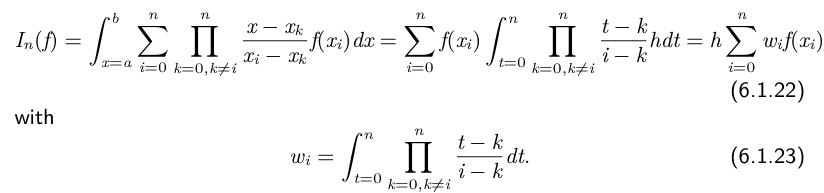
\includegraphics[width=1\textwidth]{./lagrange.png}
  
\end{figure}

and 
\begin{figure}[h!]
  \centering
     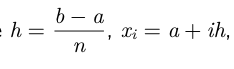
\includegraphics[width=0.4\textwidth]{./h.png}
\end{figure}

where $w_i$ can be pre-calculated and $I_n(f)$ denotes the $n'th$ order integration.
\newpage
As for composite Newton-Cotes:

\begin{figure}[h!]
  \centering
     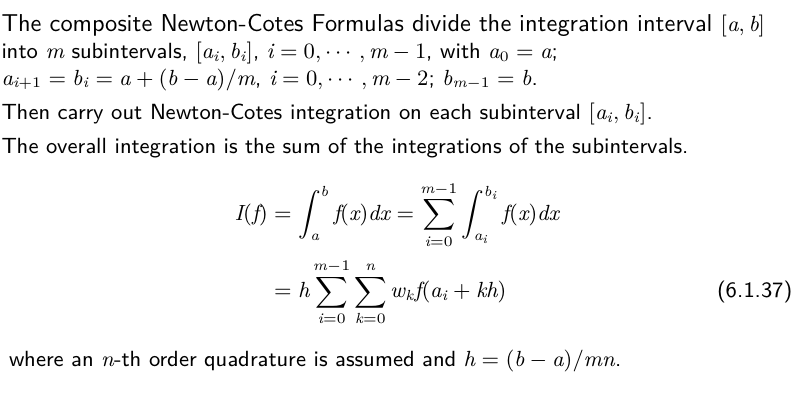
\includegraphics[width=0.98\textwidth]{./nc.png}
 \end{figure}
 Notice that the $mn$ should be exactly equal the number of intervals, so for example, if the input file is f301 then number of intervals is 300 and if $n$ is 5, then $m$ will then be $\frac{300}{5}=60$.
 
\section{Workflow}
\begin{description}  

\item [Usage:] ./hw11.out  *  $\Delta$ $<$ f*.dat, where * could be 21 or 301, $\Delta$ could be 1, 2, 4, 5 in this assignment. For example,  ./hw11.out  21 1$<$ f21.dat
\item [Solve:] N.-C. method applied on input file.
\item[Desired output:] The program will print out the result of integration in command line.
\end{description}

\section{Results}

First order Newton-Cotes integration on f301.dat is 28007.679797

\begin{center}
	\captionof{table}{N.-C. integration on f21.dat}
    \begin{tabular}{|c|c|c|}
    \hline  Order & Value &  $|Error  w.r.t. f301|$   \\
    \hline  1	&28109.399520	&101.719723	\\
    \hline  2	&28193.136660	&185.456863	\\
    \hline  4	&28161.306744	&153.626947	\\
    \hline  5	&28157.922555	&150.242758	\\\hline
     \end{tabular}
 \end{center}


\section{Plot Analysis}

\begin{figure}[h!]
  \centering
     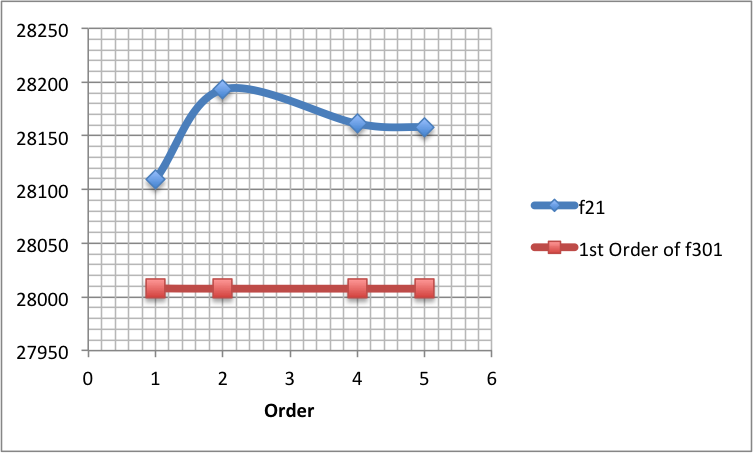
\includegraphics[width=0.9\textwidth]{./trend.png}
  \caption{Integration Values}
\end{figure}
\begin{figure}[h!]
  \centering
     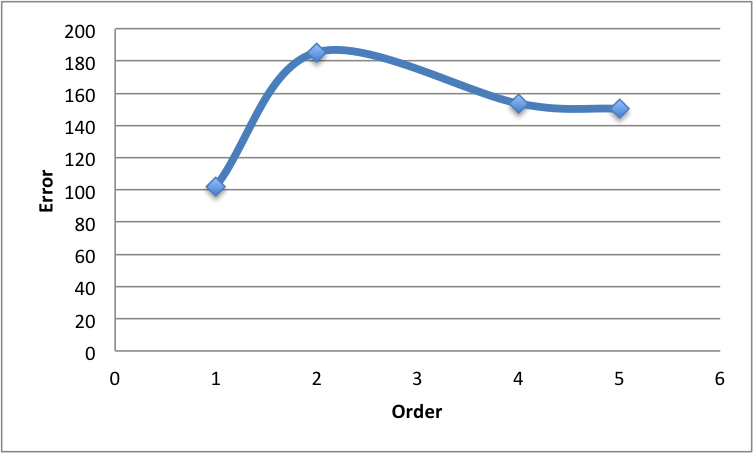
\includegraphics[width=0.9\textwidth]{./error.png}
  \caption{Error}
\end{figure}

\section{Observations}

The standard result should be 28007.679797, the result of first order N.-C. integration on f301, since f301 contains much more support points than f21 does. Knowing that trapezoidal and Simpson formulae are special instances of the Newton-Cotes formulas when order is 1 and 2, we can view the error plot to see how accurate they really are, and amazingly the result shows us that for this assignment, trapezoidal method would be the most accurate one. As for the trend, since I only did 4 orders, I can only say that the error will start declining after order of 2.


\end{document} 
